\documentclass[11pt]{article}
\usepackage[margin=1in, lmargin=0.75in]{geometry}
\usepackage{caption}
\usepackage{float}
\usepackage{graphicx}
\usepackage{latexsym}
\usepackage{amsmath}
\usepackage{cancel}
\usepackage{astro}
\usepackage{url}
\usepackage[bottom]{footmisc}

\newcommand\allbold[1]{{\boldmath\textbf{#1}}}
\newcommand\pc{\mathrm{\ pc}}
\newcommand\Lpc{\ L_\odot/\!\!\pc^2}
\newcommand\sech{\ \!\mathrm{sech}}

\begin{document}

\begin{flushright}Meredith Durbin\\
Tom Quinn\\
Astro 507: Thermodynamics\\
\today\\

\end{flushright}

\center{\textsc{Homework 1}} \\[6pt]

\begin{enumerate}

\item
    \begin{enumerate}
    \item % Specifically, address the dimensions you use for velocity, mass, energy, length, and time. Discuss how you determine if a collision has occurred, what equations you solve during a collision, and how you handle the box boundaries.
    For my particles in a box I chose a box side length of 100, particle masses and initial velocities of 1, and a timestep of 0.1. I use the \texttt{query\_pairs()} method of \texttt{scipy.spatial.cKDTree} to find all pairs of particles within twice the particle radius of each other. During a collision, I calculate the normal and tangential velocities during a collision and use those to update the particle velocities. I chose reflecting box boundaries, such that if a particle bumps into a horizontal wall the $y$-component of its velocity changes sign, and if it bumps into a vertical wall the $x$-component of its velocity changes sign.
    
    An interactive notebook (since github won't display it properly) is available at\newline \url{https://meredith-durbin.github.io/holoviews/particlesinabox}.\newline Github: \url{https://github.com/meredith-durbin/ASTR507/tree/master/HW1}.
    \item Plots for initial and final positions and velocities:
    \begin{figure}[H]
    \centering
    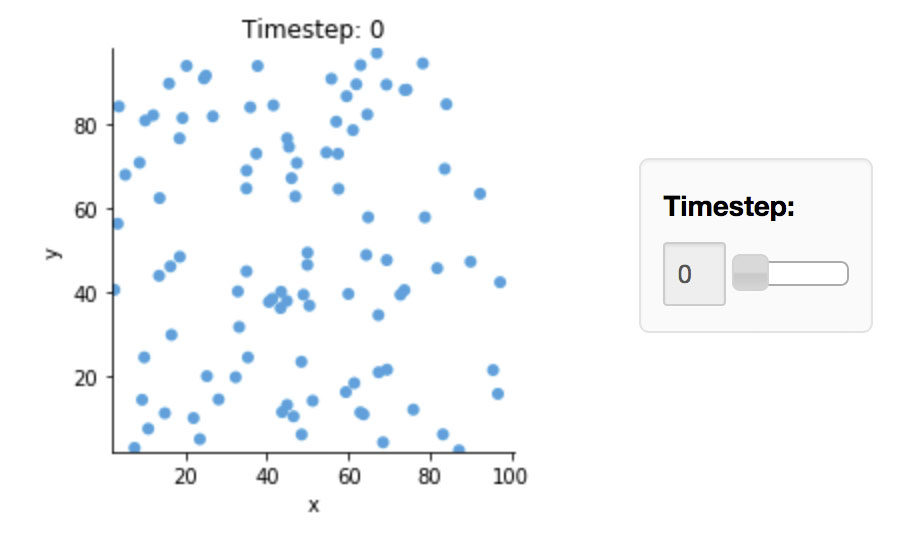
\includegraphics[width=0.4\textwidth]{position_initial.jpg}
    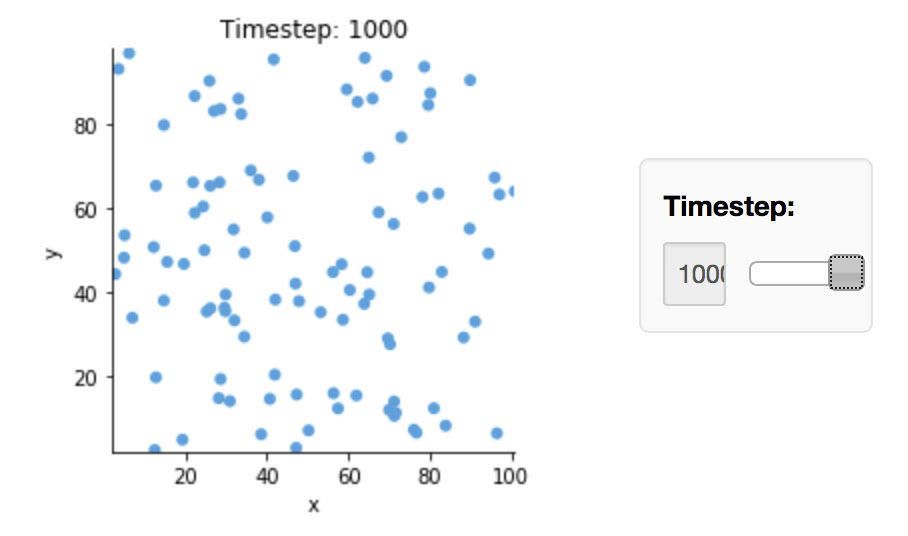
\includegraphics[width=0.4\textwidth]{position_final.jpg}
    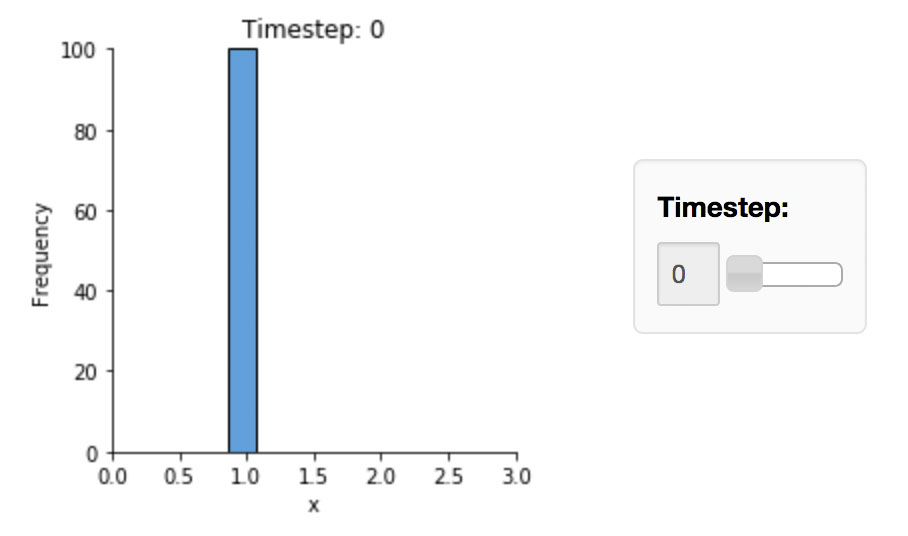
\includegraphics[width=0.4\textwidth]{velocity_initial.jpg}
    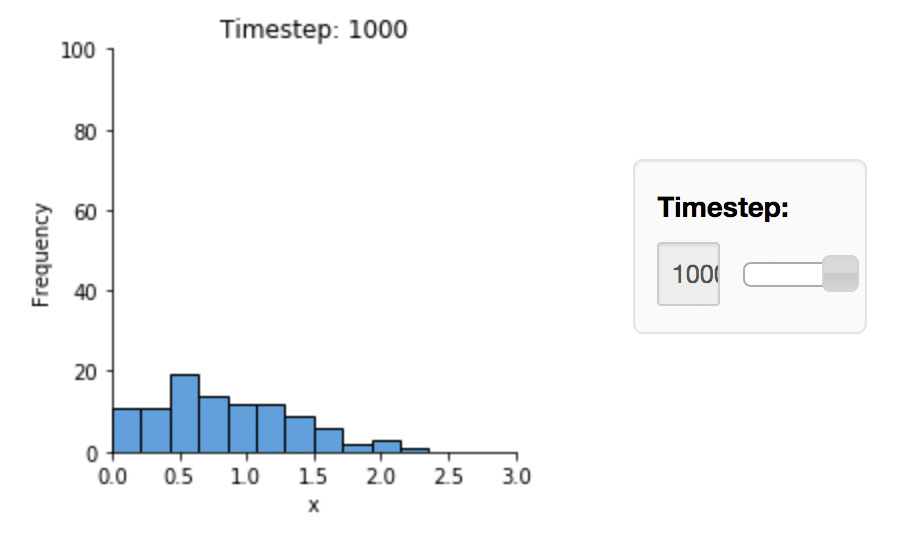
\includegraphics[width=0.4\textwidth]{velocity_final.jpg}
    \end{figure}
    \end{enumerate}
\item
    \begin{enumerate}
    \item We are given that $f(q,p) \propto e^{-E/k_BT}$.% For the velocity distribution, if we assume that $E = \frac{1}{2}m(v_x^2+v_y^2)$, then we can write:
    \begin{align}
    dN &\propto f(p)dp \\
    &= e^{-p^2/2mk_BT}dp \\
    &= e^{-(p_x^2 + p_y^2)/2mk_BT}dp_xdp_y \\
    &= e^{-m(v_x^2 + v_y^2)/2mk_BT}m^2dv_xdv_y \\
    &= e^{-mv^2/2k_BT}m^2v dv d\theta
    \end{align}
    Integrating this over all $\theta$ and rearranging, we arrive at $dN/dv \propto 2\pi e^{-mv^2/2k_BT}m^2v$. To find the normalization constant, we want this to integrate to one over all velocities.
    \begin{align}
    1 &= C \int_0^\infty e^{-mv^2/2k_BT}m^2v dv \\
    %&= 2\pi C \frac{m}{k_BT} \\
    C &= \frac{m}{2\pi k_B T}
    \end{align}
    From this we find the Maxwellian velocity distribution, $dN/dv = \frac{m}{2\pi k_BT} v e^{-mv^2/2k_BT}$.
    
    For the energy distribution, we have $dN/dE \propto e^{-E/k_BT}$. It is easy to see that this normalizes simply to $dN/dE = \frac{1}{k_BT}e^{-E/k_BT}$.
    \item Maxwellian velocity distribution overplotted on results coadded from 100 simulation runs:
    \begin{figure}[H]
    \centering
    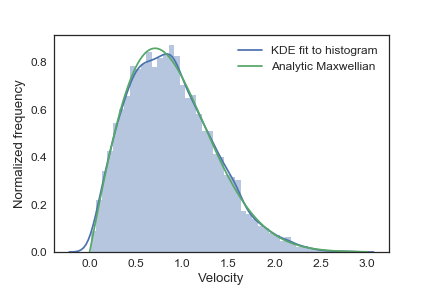
\includegraphics[width=0.6\textwidth]{maxwellian.png}
    \end{figure}

    \item Two Maxwellian velocity distributions overplotted on results coadded from 100 simulations with half the particles at m=1 and half at m=10:
    \begin{figure}[H]
    \centering
    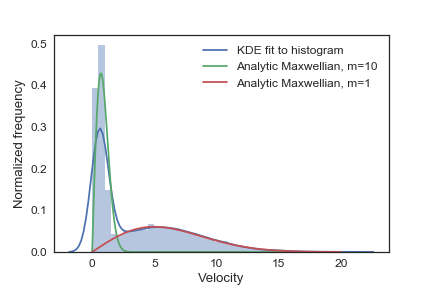
\includegraphics[width=0.6\textwidth]{maxwellian_2.png}
    \end{figure}
    \end{enumerate}
\item 
    \begin{enumerate}
    \item A simple numerical criterion for relaxation would be to calculate the difference between the 50th percentile of the particle velocities and the theoretical 50th percentile of the Maxwellian velocity distribution.
    \item The relaxation time $t_\mathrm{relax}$ for a given particle is dependent on the mean free path and initial velocity $v_0$. The mean free path is the inverse of the cross section times the number density, $1/\sigma n$. Therefore, $t_\mathrm{relax} = 1/\sigma n v_0$. (For two dimensions, $\sigma$ is the particle diameter, assuming circular particles.)
    \item Plots of relaxation time by number density and radius:
    \begin{figure}[H]
    \centering
    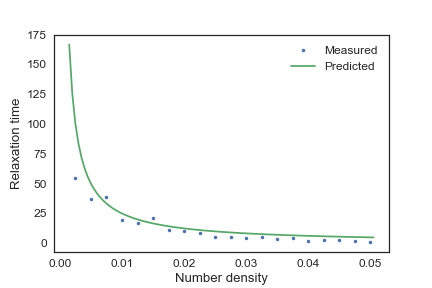
\includegraphics[width=0.6\textwidth]{trel_n.png}
    \end{figure}
    \begin{figure}[H]
    \centering
    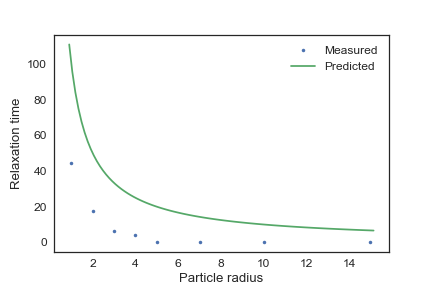
\includegraphics[width=0.6\textwidth]{trel_r.png}
    \end{figure}

    \end{enumerate}

\end{enumerate}
\end{document}